\section{Results} \label{sec:results}

\begin{figure}[ht]
\vskip 0.2in
\begin{center}
    \centerline{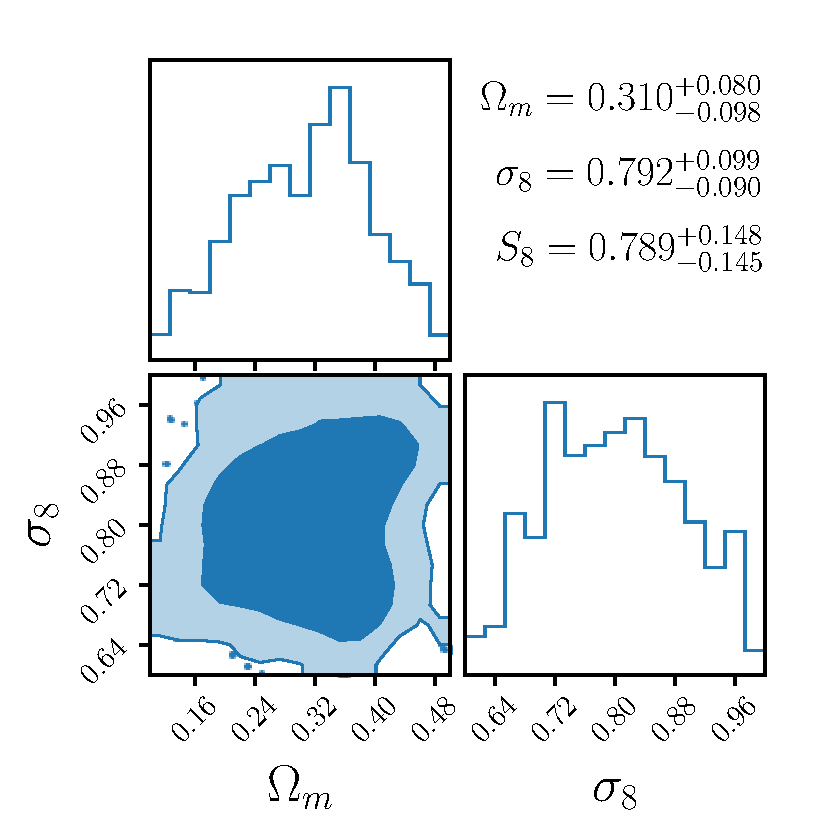
\includegraphics[width=0.9\columnwidth]{figs/p_oms8_x.pdf}}
    \caption{    }\label{fig:p_omega_x}
\end{center}
\vskip -0.2in
\end{figure}

Our posterior on $\Omega_m$ and $\sigma_8$ is inferred assuming a galaxy
formation model and a SED model. 
This is illustrated in Eq.~\ref{eq:post0} where $p(\Omega, B\given\theta^g_i)$
is determined by the galaxy formation model and
$p(\theta^g_i\given {\bfi X}_i)$ is determined by the SED model.  
Below we discuss the caveats of these assumptions and how they can be accounted
for in future research.

\subsection{Galaxy Formation Model} \label{sec:galmodel}
Some interpretation of cosmology with one galaxy here and what that may
actually imply for $p(\Omega, B\given\theta^g_i)$


\subsection{SED Modeling} \label{sec:sed}
The forward modeled photometry for the simulated galaxies in our training data
are constructed using SED modeling (Section~\ref{sec:sims}. 

dust modeling is unrealistic, which could bias the inferred $\theta^g$

emission lines are crap

hard assumptions on the IMF

Despite these serious limitations, we can identify subpopulations of galaxies
that are the least sensitive to them.
For example, quiescent galaxies do not have emission lines and we can identify
ones without dust attenuation from XXXX (galaxy zoo? emission lines?).  
Furthermore, recent studies using both lensing and IR spectral features also
find no IMF variations in the bulk populations of nearby quiescent galaxies. 
%[79] Smith, R. J., Lucey, J. R., & Conroy, C. 2015a, MNRAS, 449, 3441 [80]
%Smith, R.J., Alton, P., et al. 2015b, MNRAS, 454, L71, Myers, A. T., McKee, C. F., et al. 2013, ApJ, 766, 97
Hence, although $p(\theta^g_i\given {\bfi X}_i)$ is not robust over the full
space of ${\bfi X}$, it is robust for dustless quiescent galaxies.

In principle, $p(\Omega, \mathcal{B}\given {\bfi X_i}) = \int p(\Omega,
\mathcal{B}\given \theta^g_i)\,p(\theta^g_i \given {\bfi X_i})\,{\rm
d}\theta^g_i$, where $\theta^g_i$ is a latent variable that is marginalized. 
